\documentclass[10 pt, a4paper]{article}

\usepackage{graphicx}
\usepackage{caption}
\usepackage{anysize}
%\usepackage{changepage}
\usepackage{amsfonts}
\usepackage{float}
\usepackage{todonotes}
\usepackage{amsmath}
\usepackage[toc,page]{appendix}
\usepackage{subcaption}
\usepackage{hyperref}

\marginsize{2 cm}{2 cm}{1 cm}{2 cm}

\captionsetup[figure]{labelfont=bf,textfont=it,width=0.88\textwidth}
\captionsetup[table]{labelfont=bf,textfont=it,width=0.88\textwidth}

\setlength{\parindent}{0 cm}

\title{
 Studying the Phase Transition in the Ferromagnetic Square-Lattice 2D Ising Model using Monte Carlo Algorithms and Convolutional Neural Networks  \\
  \Large Computational Physics Project 2
}

\author{Tim Koreman (s2418541)}


\begin{document}

\maketitle


\abstract{Monte Carlo algorithms can be used to study the Ising model. In this report we look at the phase transition in the ferromagnetic zero field
 2D square lattice Ising model by calculating the magnetisation per spin, the specific heat per spin and the susceptibility per spin at a range of temperatures. For those observables the behaviour around the critical temperature has a distinct shape that agrees with results from literature \cite{thijssen}. When we look at the effect the lattice size on those shapes we see that they become sharper and more defined for bigger lattice sizes which agrees with the expectation that bigger lattice sizes approach the thermodynamics limit.
\\
\\
A second method used to look at the phase transition is by using a Convolutional Neural Network. Using such a  class of a Artificial Neural Network a value for the critical temperature of $T_C = 2.23(5)$ was found which agrees with the analytical result.
}


\section{Introduction}

Many thermodynamic systems demonstrate a phase transition along some order parameter. One of the simplest systems which demonstrate such a transition is the Ising model. This system consists of N spins with value $-1$ or $1$ arranged on some lattice and has a phase transition at some finite temperature. In this report we look at this phase transition by looking the average magnetisation, heat capacity per spin and the susceptibility per spin at a range of temperatures using Monte Carlo algorithms.
\\
\\
Monte Carlo algorithms are the conventional method to computationally study the Ising model. In Recent years Artificial Neural Networks have become a popular method for data analysis. Using this method we try to find the critical temperature of the phase transition.


\section{Theoretical Background} \label{sec:theo}

\subsection{Ising Model}

The Hamiltonian of the Ising model is given by

\begin{align*}
H = - J \sum_{\langle i,j\rangle} s_i s_j - H \sum_i s_i
\end{align*}

Where $J$ is a coupling constant, $s_i$ the spin value at site $i$, $\sum_{\langle ij\rangle}$ the sum over the nearest neighbours and $H$ the magnitude of an external magnetic field. In order to reduce the complexity of the phase transition we look at the zero field case where $H = 0$ so the Hamiltonian becomes

\begin{align*}
H = - J \sum_{\langle i,j\rangle} s_i s_j 
\end{align*}

where when $J > 0$ the systems favour ferromagnetism and when $J < 0$ anti ferromagnetism. The Ising model has a phase transition at a finite temperature. Analytically it can be found that the critical temperature is at $k_B T_C / J = \frac{2}{\ln(1 + \sqrt{2})} \simeq 2.2691 \dots $ \cite{onsager}.

\subsection{Single flip Monte Carlo algorithms}

In order to simulate the system at a given temperature we look at two single flip Monte Carlo algorithms, the metropolis algorithm and the heat bath algorithm. In the metropolis algorithm a random spin is flipped and the change in energy that flip would cause is evaluated. If this change is negative than it is accepted outright, if it is positive it is accepted with a probability $P$ given by

\begin{align} \label{metropolis}
P = \exp(-\beta \Delta H)
\end{align}

where $\beta = \frac{1}{k_B T}$ with $k_B$ the Boltzmann constant and $T$ the temperature and $\Delta H$ the change in energy. In the heat bath algorithm a random spin is flipped and it is accepted with a probability $P$ given by

\begin{align}
P = \frac{1}{1 + \exp(\beta \Delta H)}
\end{align} 

where $\beta = \frac{1}{k_B T}$ with $k_B$ the Boltzmann constant and $T$ the temperature and $\Delta H$ the change in energy.
\\
\\
In order to calculate observables from the system we first need to let it equilibrate. In order to evaluate the equilibration time we simulate the system and calculate the magnetisation every step. In this context we use a step size of N flips. When we look at the equilibration for the metropolis algorithm in figure \ref{fig:metro} we can see that after 20 steps the magnetisation fluctuates around the same value. When we do the same for the heat bath algorithm (see figure \ref{fig:heat}) we see that it takes almost 40 steps for the heat bath algorithm to reach equilibration. Therefore the metropolis algorithm is used for the calculation of the observables.

\begin{figure}[H] 
\begin{subfigure}[b]{0.5\textwidth}
\begin{figure}[H]
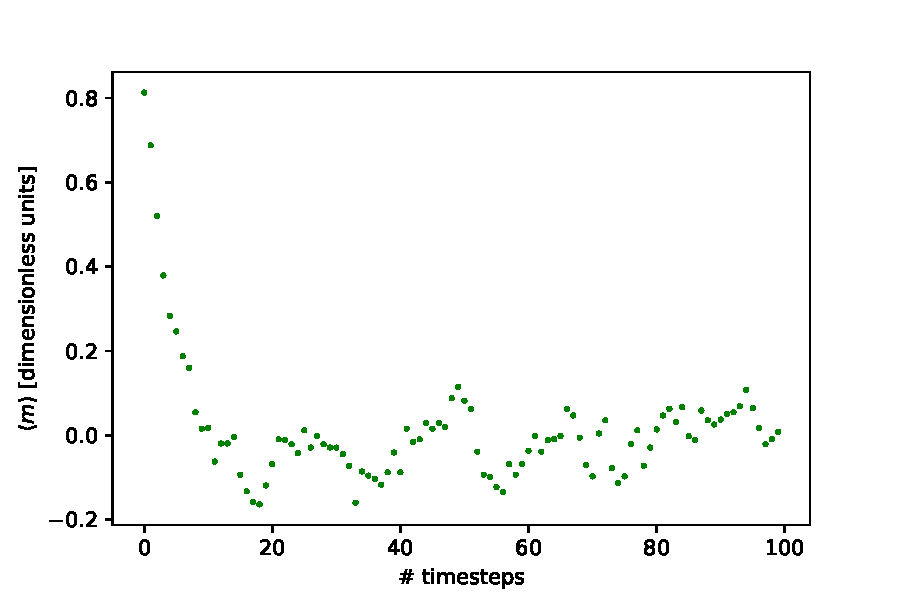
\includegraphics[width=\textwidth]{timeMC}
\caption{Metropolis algorithm. \label{fig:metro}}
\end{figure}
\end{subfigure}
\begin{subfigure}[b]{0.5\textwidth}
\begin{figure}[H] 
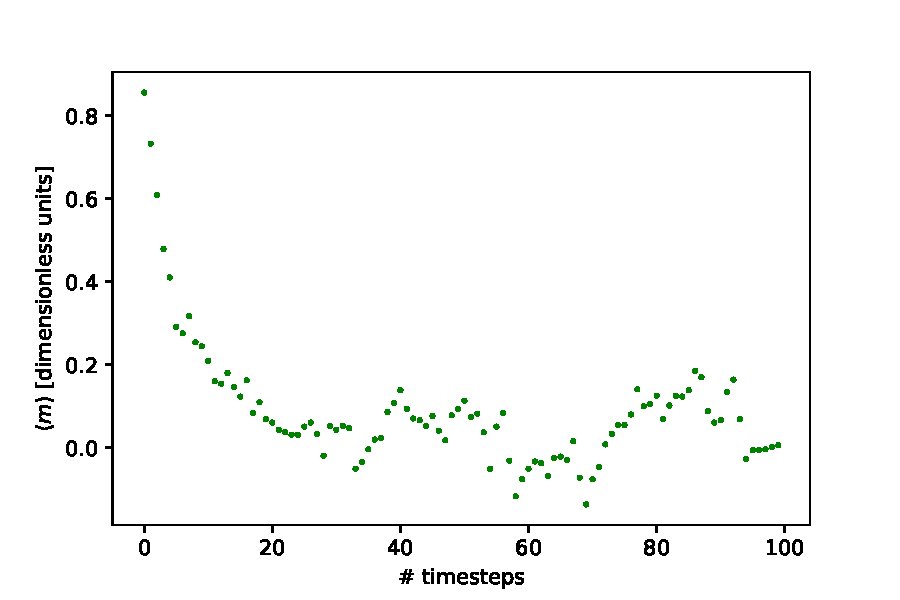
\includegraphics[width=\textwidth]{timeHeatbath}
\caption{Heat bath algorithm. \label{fig:heat}}
\end{figure}
\end{subfigure}
\caption{Magnetisation vs. the number of timesteps for a $32 \times 32$ lattice using the metropolis algorithm and the heat bath algorithm  at $\frac{k_B}{J} T = 3.6$. 1 step contains 1024 spin flips.} 
\end{figure}


\subsection{Observables}

After the system has reached equilibration we can start to sample to system in order to calculate the observables. The system is sampled every time step, where 1 time step is defined as being N flip attempts. From these samples the magnetisation per spin $m$ defined by 

\begin{align}
\langle m \rangle = \frac{1}{N} \langle \sum_i s_i\rangle
\end{align}

where $\langle \dots \rangle$ is used to denote the ensemble average, $N$ the number of spins and $s_i$ the spin at site $i$ can be calculated. From this magnetisation the susceptibility per spin $\chi$ defined by

\begin{align}
\chi = \beta N \left( \langle m^2 \rangle - \langle m \rangle^2 \right)
\end{align}

where $\beta = \frac{1}{k_B T}$ with $k_B$ the Boltzmann constant and $T$ the temperature, $N$ the number of spins and $\langle m^2 \rangle - \langle m \rangle^2$ the variance of the magnetisation can be calculated. The third observable calculated is the specific heat per spin $c$ defined by

\begin{align}
c = \frac{k_B \beta^2}{N} \left( \langle E^2 \rangle - \langle E \rangle^2 \right)
\end{align}

where $\beta = \frac{1}{k_B T}$ with $k_B$ the Boltzmann constant and $T$ the temperature, $N$ the number of spins and $\langle E^2 \rangle - \langle E \rangle^2$ the variance of the energy.

\subsection{Artificial Neural Networks}

Artificial Neural Networks (ANN) are a method to study data loosely inspired by biological neurons. An ANN consists of a collection of connected nodes grouped in layers. Each of those nodes takes the input from (a part of) the previous layer, multiplies it by a set of weights $w$, applies an activation function to the result and feed that result to the next layer. In order to determine this set of weights the ANN is applied to a large dataset for which the desired outputs are known. In this process called training the ANN is repeatedly applied to this dataset, updating the weights each time until the accuracy reaches an equilibrium. Each of those runs over the dataset is often called an epoch.
\\
\\
One of the simplest examples of an ANN is the single-layer perceptron. In such a system there are 2 layers, a input layer and a output layer. The input layer consists of a input vector $x_n$. Each node in the output layer takes that input vector and takes the dot product with its weight vector $w_n$. To the resulting scalar we apply the activation function. For this activation function there are many choices, e.g. the sigmoid function. 
\\
\\
This simple class of a Neural Network already performs better at certain tasks such a pattern recognition in images then hand written code to solve those problems. A type of networks that is a bit more complex but more suited for image pattern recognition is the Convolutional Neural Network (CNN). Such a network starts with applying one or more convolutional layers before feeding it to a so called fully connected layer\footnote{Called fully connected because each node in the input layer is connected to each node in the following layer which is not the case for the CNN.} that resembles the single layer perceptron  described earlier.

\begin{figure}[H]
\centering
%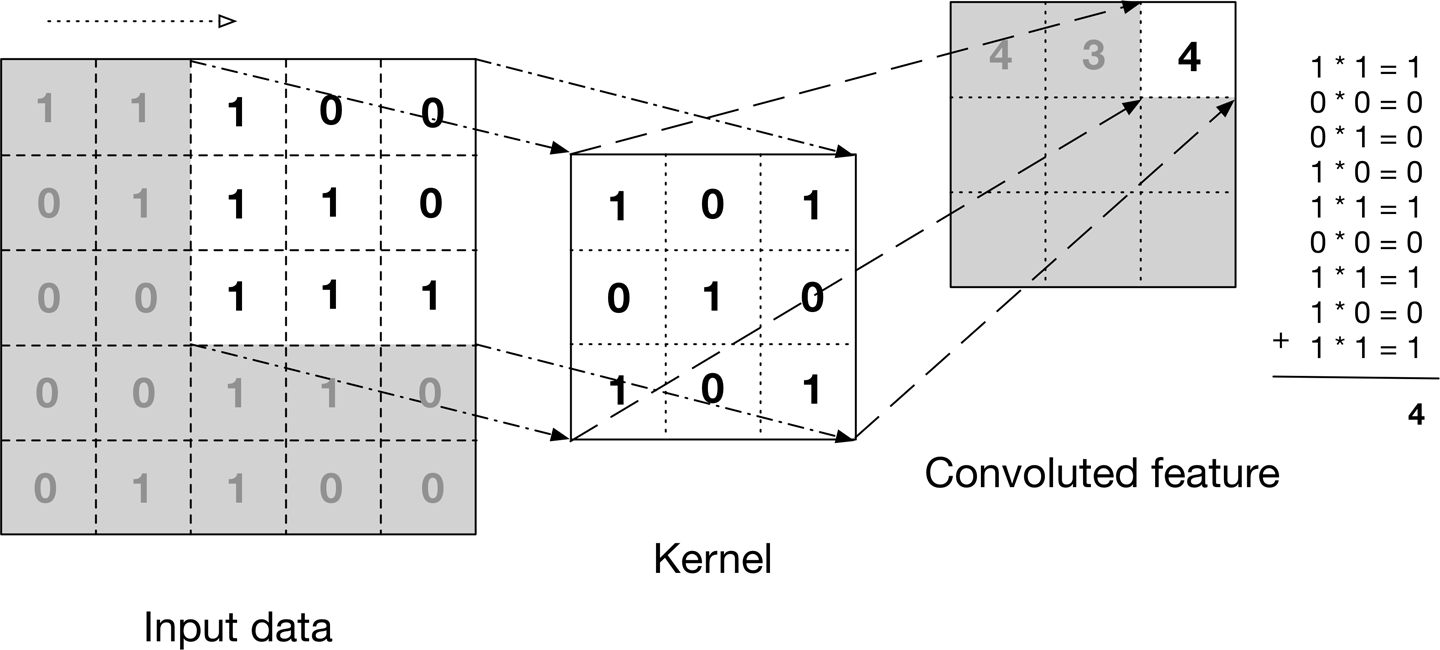
\includegraphics[width=0.7\textwidth]{CNNop}
\todo[inline]{Sourced image removed.}
\caption{Example of the operation of a single convolutional layer. Source: \cite{deep}. \label{fig:CNNop}}
\end{figure}

Such a convolutional layer uses a kernel with size $s \times s$ that moves across the image (figure \ref{fig:CNNop}). Each time this kernel is applied to the image from the previous layer it takes $s \times s$ values from the image from the previous layer, multiplies each value with a set of weights and apply an activation function to it. This result forms a part of the image for the next layer. This kernel moves across the image in steps with a size that is often called the stride of the kernel.
\\
\\
These convolutional layers reduce the size of the image with each layer. When the size is reduced enough a fully connected layer is used for the final classification. How many layers of each type should be used is often more of an art than a science and is often determined using trial and error.
\\
\\
This process, often used for image classification, can be used to study the Ising model. One way of studying the Ising model with a CNN could as a thermometer, ie. feed the CNN a labelled collection of equilibrated Ising lattices and let it determine the temperature at which they were generated. The final result from this process would be to find the value of the critical temperature from this process.\footnote{ Using more complicated ANNs more aspects of the Ising model such as the observables can be studied, see for example Torial \& Meiko 2016 \cite{IsingRBM}}


\section{Methods} \label{sec:meth}

\subsection{Metropolis simulation setup} \label{sec:simsetup}

In order make the numerical values in the simulation more manageable we define dimensionless units given in table \ref{tab:natunits}.

\begin{table}[H] 
\centering
\caption{Definition of the dimensionless units as used in the simulation. All plots and results given are in natural units where the tilde is dropped for notational clarity.  \label{tab:natunits}}
\begin{tabular}{l}
Natural Units:                                     \\ \hline
$\tilde{T} =  \frac{k_B}{J} T$                     \\
$\tilde{c} = \frac{1}{k_B} c$                   \\
\end{tabular}
\end{table}

The system was initialized with all spins aligned with value $1$.
\\
\\
We want to eliminate edge effects therefore we use periodic boundary conditions. We calculate the observables by sampling our system $n$ times and replacing the ensemble average with time averages. To calculate the errors for these observables bootstrapping is used. Bootstrapping re-samples with replacement from the $n$ samples took from the system and the observables are calculated for each of those steps. This process repeated $N_{\mathrm{bootstrap}}$ times and using the $N_{\mathrm{bootstrap}}$ values found for the observables the error $\sigma_O$ for an observables $O$ calculated using

\begin{align*}
\sigma_O = \sqrt{\langle O ^2 \rangle - \langle O \rangle ^2}
\end{align*}.



\subsection{Convolutional Neural Network setup}


In order to prepare the data for the CNN we use the Monte Carlo simulation used for determining the observables. We let the system equilibrate and then save the array with the value of each of the spins as a vector with length $L \times L$ and in a separate list the temperatures at which those lattices were generated. This was done at a range of temperatures from $T = 0.1$ to $T = 4.5$ with $\Delta T = 0.001$ to generate a set of 4400 labelled lattices around the critical temperature. These lattices had $80 \times 80$ spins. These lattices were fed to the CNN to train it.  
\\
\\
The CNN was trained to classify the lattices into a set of temperature classes. These classes are defined using the inverse temperature $\beta$ around the critical temperature. We choose a range of classes from $\beta = 0.22$ to $\beta = 1$ and we define 100 classes in this range.
\\
\\
The CNN used to classify the lattices had a single convolutional layer with a kernel size of 25 and a stride of 13 with the linear rectifier defined by

\begin{align}
f(x) = \mathrm{max}(0,x)
\end{align}

as the activation function. The result of this layer is than fed into a single fully connected layer with the 100 classes defined above with the softmax function defined by

\begin{align}
\sigma(\vec{z}) = \frac{e^{z_i}}{\sum_{j=1}^K e^{z_j}}
\end{align}

as the activation function. Where $i$ denotes the class it is calculated for so it has the effect of a normalized exponential function. 

\subsection{Validity Checks}

In order to validate the simulation we look at the magnetisation. For $J$ positive we expect ferromagnetic behaviour where the magnetisation at low temperature goes to $\pm 1$ and at high temperature goes to zero. In figures \ref{fig:magval} \& \ref{fig:lattices} we can see that the simulation satisfies this validity check.

\begin{figure}[H]
\centering
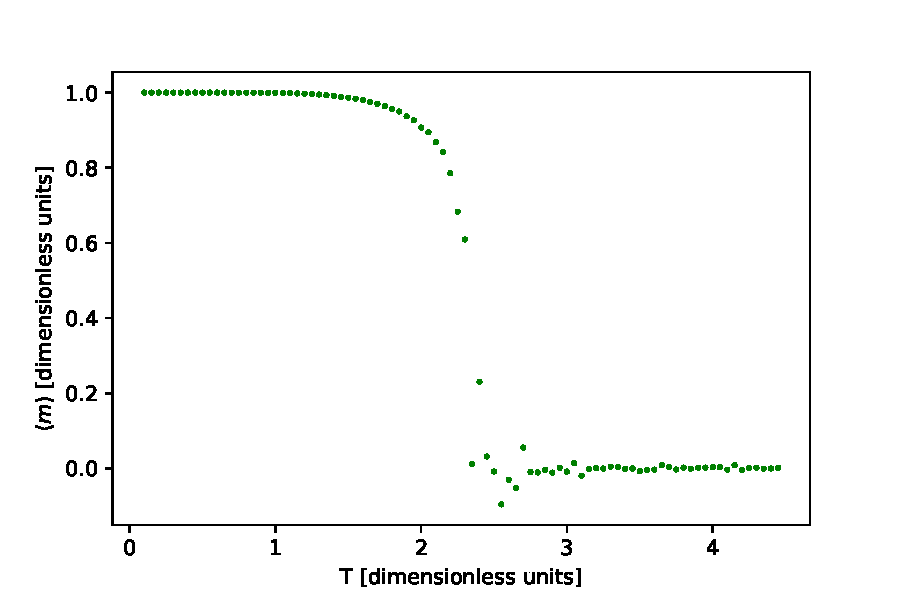
\includegraphics[width=0.7\textwidth]{magval}
\caption{Magnetisation vs. dimensionless temperature with for a system with $32 \times 32$ spins and $J > 0$. Parameters as in table \ref{tab:params}. At low temperatures the magnetisation goes to 1, at high temperatures the magnetisation goes to zero satisfying the validity check. \label{fig:magval}}
\end{figure}

\begin{figure}[H] 
\begin{subfigure}[b]{0.33\textwidth}
\begin{figure}[H]
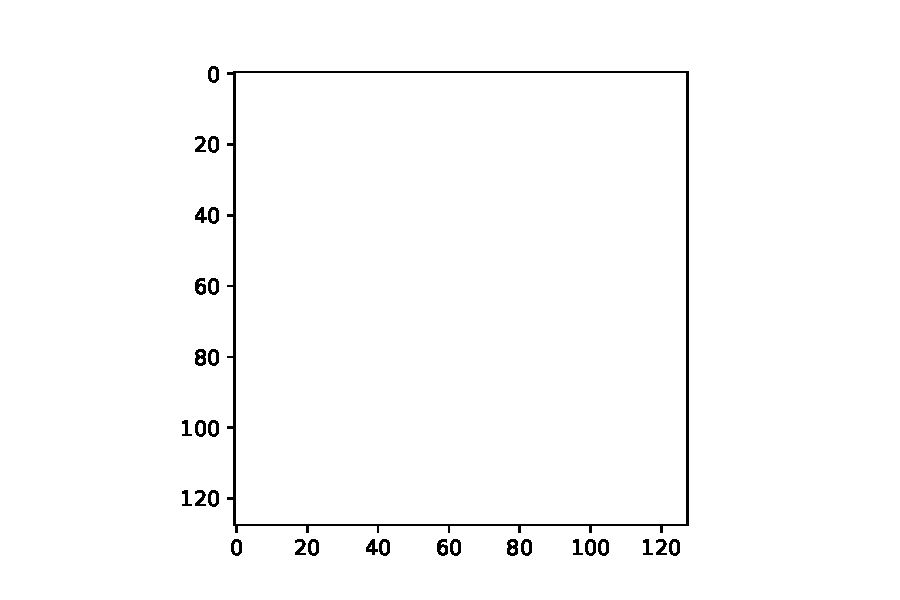
\includegraphics[width=\textwidth]{lattice128a}
\caption{$T = 0.1$.}
\end{figure}
\end{subfigure}
\begin{subfigure}[b]{0.33\textwidth}
\begin{figure}[H]
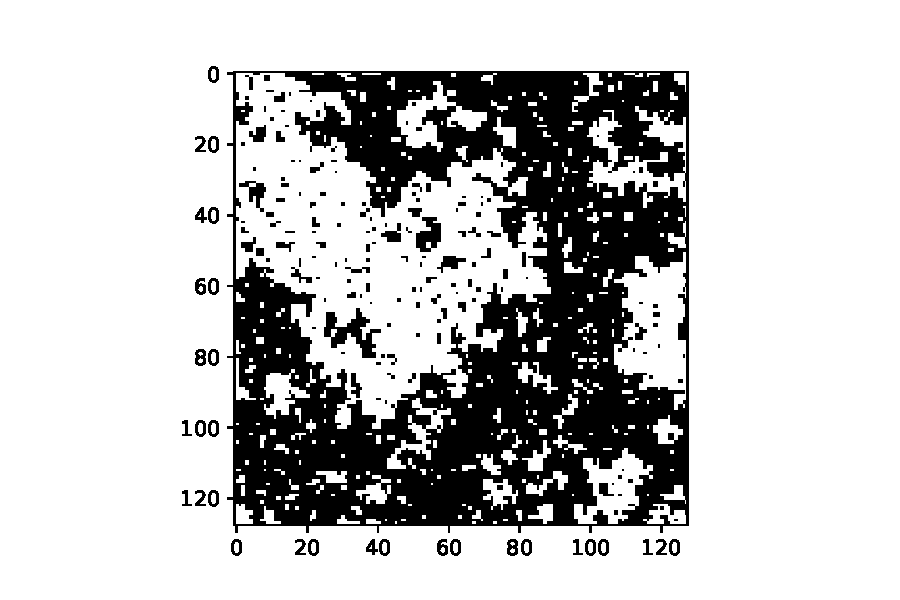
\includegraphics[width=\textwidth]{lattice128b}
\caption{$T = 2.2$.}
\end{figure}
\end{subfigure}
\begin{subfigure}[b]{0.33\textwidth}
\begin{figure}[H] 
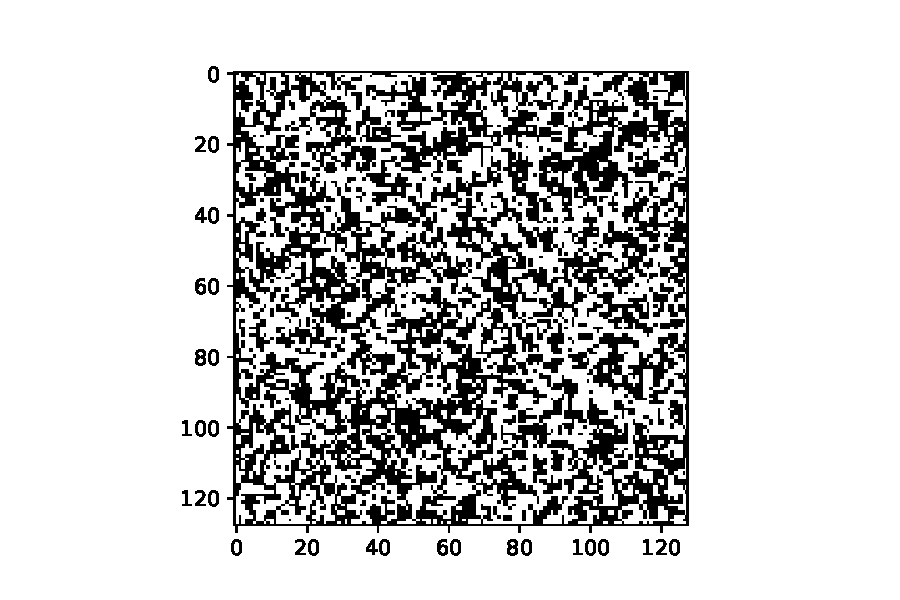
\includegraphics[width=\textwidth]{lattice128c}
\caption{$T = 4.5$.}
\end{figure}
\end{subfigure}
\caption{Ising configurations at three temperatures below, around and above the critical temperature respectively. System size of $128 \times 128$ spins. Below the critical temperature all the spins are aligned, above the critical temperature the spins are random which results in zero net spin. }
\label{fig:lattices}
\end{figure}

In order to verify whether the CNN manages to represent the phase transition we look at the weight matrix of the final, fully-connected, layer. In figure \ref{fig:weightscnn} we can see that there is indeed some phase transition in this weight matrix. 

\begin{figure}[H]
\centering
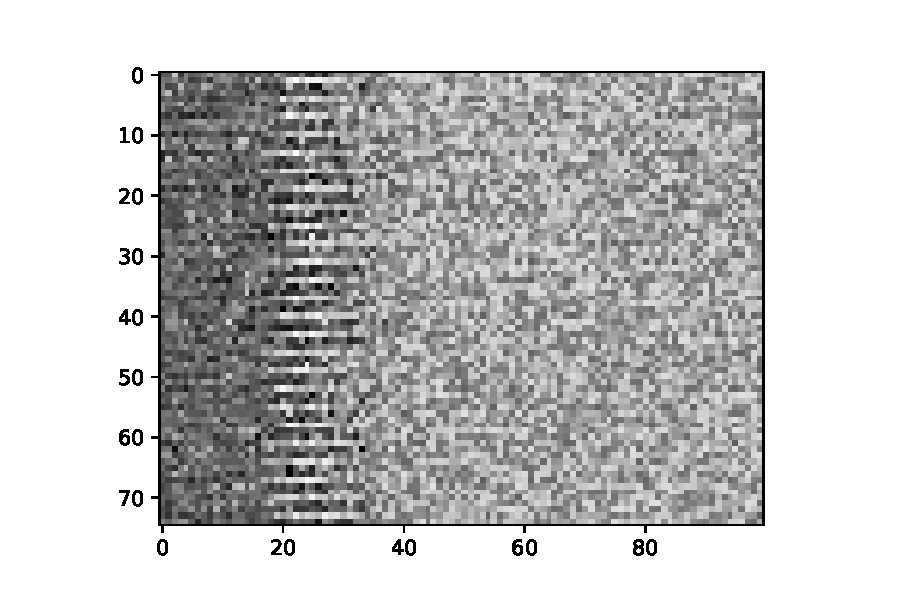
\includegraphics[width=0.7\textwidth]{weights}
\caption{Heat plot of the weight matrix of the final fully connected layer of the network, around the critical inverse temperature a phase transition can be seen. \label{fig:weightscnn}}
\end{figure}

\subsection{Implementation}

The main simulation was implemented in Visual C\# 6.0. The plots were made in Python 3.6.3 using MatPlotLib 2.1.0. The CNN was implemented using Keras 2.2.4 using the TensorFlow 1.13.1 backend in Python 3.6.3.


\section{Results} \label{sec:results}

\subsection{Observables}

For the results the algorithm as described in section \ref{sec:theo} and section \ref{sec:meth} was performed, the system was sampled and the observables were calculated using the parameters given in table \ref{tab:params}. 


\begin{table}[H]
\centering
\begin{tabular}{l|l}
Parameter: & Value:                                           \\ \hline
$n$ & $10000$       \\
$N_\mathrm{bootstrap}$          & $10$                                   \\
$\Delta T$          & $0.1$         \\                                   
\end{tabular}
\caption{Parameters used in the simulations runs used to generate the plots. \label{tab:params}}
\end{table}

The simulations were run with $J > 0$ so we expect ferromagnetic behaviour above and below the critical temperature. For the magnetisation per spin we expect it to go to $\pm 1$ at low temperatures and to 0 for high temperatures. In figure \ref{fig:mag128} we see that the simulation behaves as expected. 

\begin{figure}[H]
\centering
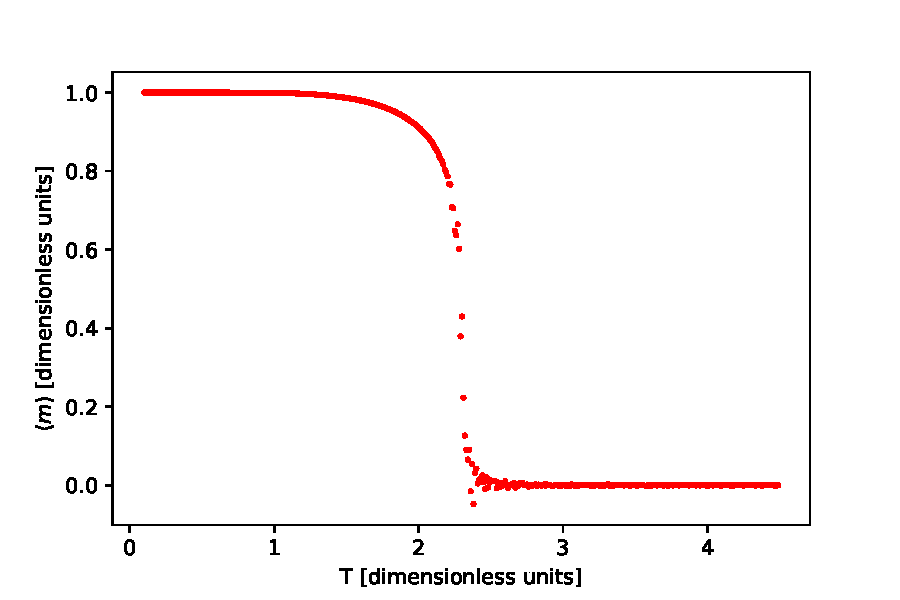
\includegraphics[width=0.7\textwidth]{mag128}
\caption{Magnetisation per spin vs. dimensionless temperature with for a system with $128 \times 128$ spins and $J > 0$.Parameters as in table \ref{tab:params}. Errors calculated using the bootstrap method. \label{fig:mag128}}
\end{figure}

For the specific heat per spin we expect a discontinuity at the phase transition in the thermodynamic limit. For a finite size system we expect a peak at the critical temperature that becomes sharper the bigger the system becomes. In figure \ref{fig:cv128} we see that a system of $128 \times 128$ spins has sharp peak at the critical temperature. In figure \ref{fig:cv} we see that for smaller systems the peak becomes less sharp and more spread.

\begin{figure}[H]
\centering
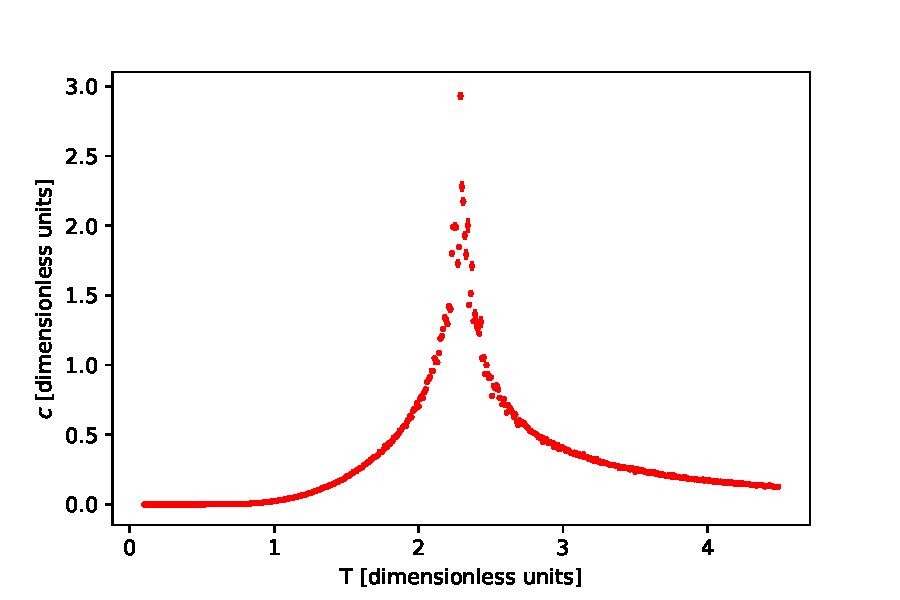
\includegraphics[width=0.7\textwidth]{cv128}
\caption{Specific heat per spin vs. dimensionless temperature with for a system with $128 \times 128$ spins and $J > 0$. Parameters as in table \ref{tab:params}. Errors calculated using the bootstrap method. \label{fig:cv128}}
\end{figure}

\begin{figure}[H]
\centering
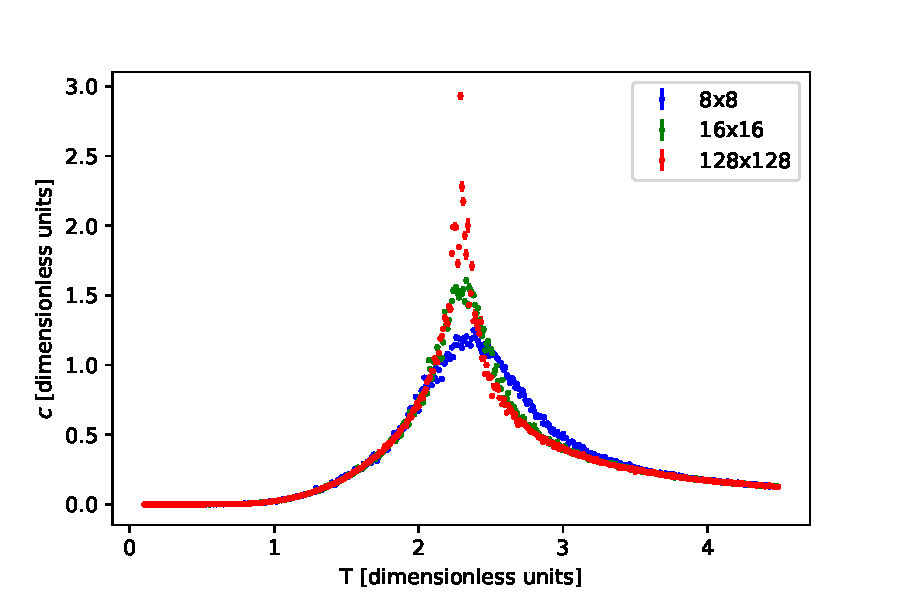
\includegraphics[width=0.7\textwidth]{cv}
\caption{Susceptibility per spin vs. dimensionless temperature with for a system with $128 \times 128$ spins and $J > 0$. Parameters as in table \ref{tab:params}. Errors calculated using the bootstrap method. \label{fig:cv}}
\end{figure}

We expect the susceptibility per spin to go to zero far above and below the critical temperature and to have a peak at the phase transition in the thermodynamic limit. In figure \ref{fig:chi128} we see the susceptibility per spin for a system with $128 \times 128$ spins and see that it has a peak at the critical temperature. In figure \ref{fig:chi} we see that this peak becomes broader for smaller system sizes. 

\begin{figure}[H]
\centering
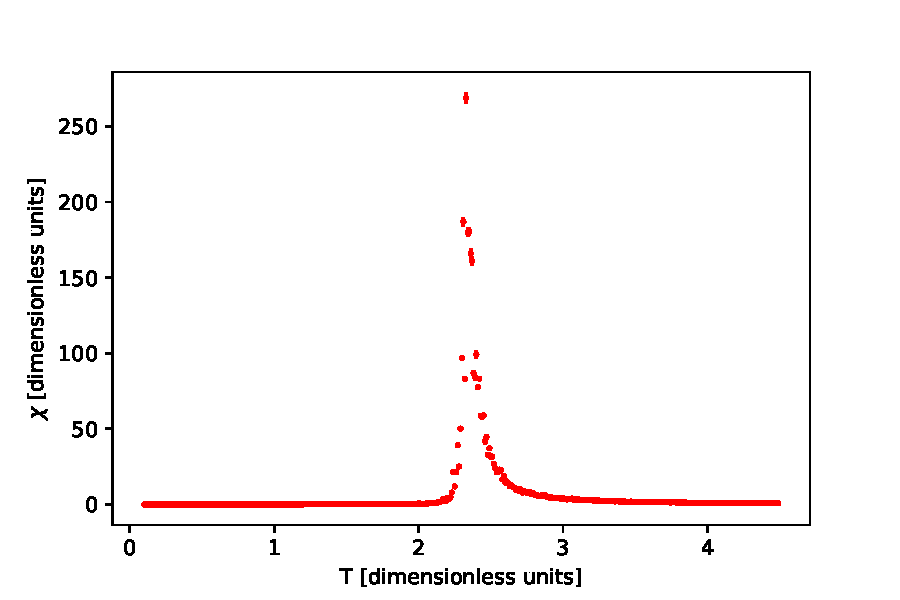
\includegraphics[width=0.7\textwidth]{chi128}
\caption{Susceptibility per spin vs. dimensionless temperature with for a system with $128 \times 128$ spins and $J > 0$. Parameters as in table \ref{tab:params}. Errors calculated using the bootstrap method. \label{fig:chi128}}
\end{figure}

\begin{figure}[H]
\centering
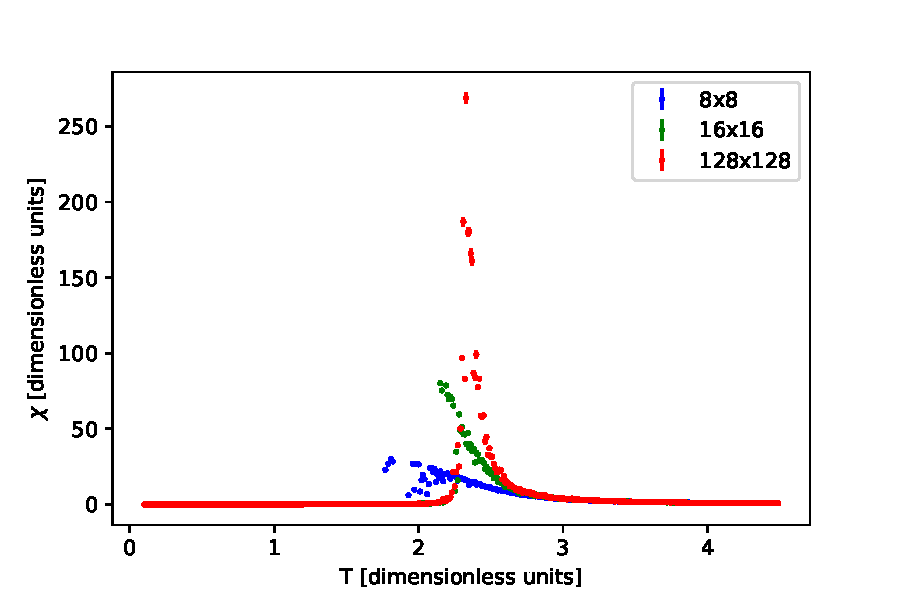
\includegraphics[width=0.7\textwidth]{chi}
\caption{Susceptibility per spin vs. dimensionless temperature with for a system with $128 \times 128$ spins and $J > 0$. Parameters as in table \ref{tab:params}. Errors calculated using the bootstrap method. \label{fig:chi}}
\end{figure}

\subsection{Critical temperature using CNN}

In order to determine the temperature at which the phase transition in the weights (figure \ref{fig:weightscnn}) of the CNN occurs  we look at the sum of all the weights for each class (see figure \ref{fig:fit}). In order to quantify the temperature of the transition we fit a function to the data points. Inspired by Tanaka \& Tomiya 2017 \cite{phasemethod} we use the function

\begin{align*}
W(x) = a \tanh(c(x - \beta_C)) - b
\end{align*}

with $a,b,c,\beta_C$ the fitting parameters where $\beta_C$ corresponds with the inverse critical temperature. The fit in figure \ref{fig:fit} gives a value of $\beta_C = 0.449(9)$ which results in $T_C = 2.23(5)$ which agrees with the analytical result. The error in this expectation value was calculated from the covariance matrix of the fit, no error was calculated for the weights in the network.

\begin{figure}[H]
\centering
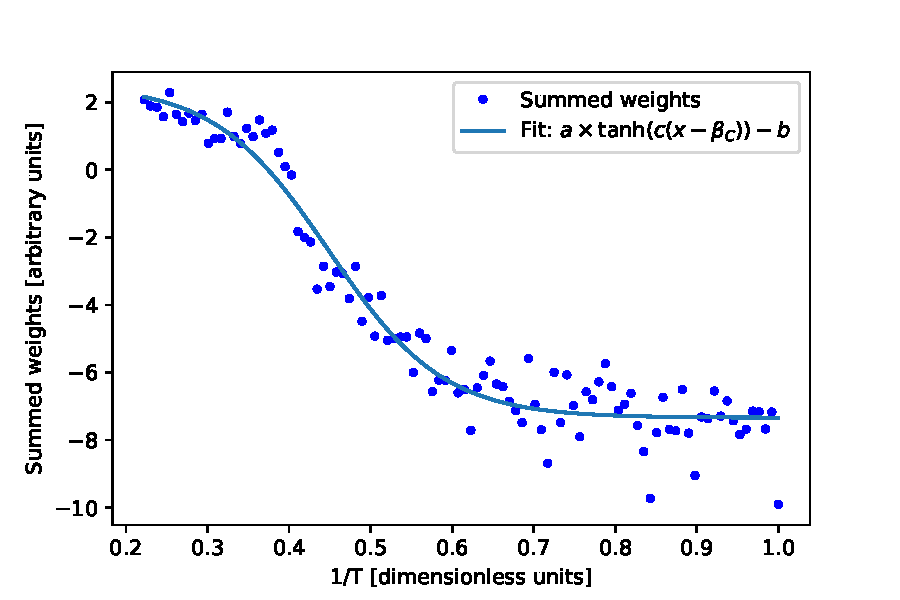
\includegraphics[width=0.7\textwidth]{fit}
\caption{Sum of the weights for each of the classes with the fitted $\tanh$ function. The critical inverse temperature for this fit has a vlaue of $\beta_C = 0.449(9)$. \label{fig:fit}}
\end{figure}

This result was acquired after running the CNN for 300 epochs. After these 300 epochs the CNN manages to correctly classify the temperature for 25\% of the data. This low accuracy could be explained by the overlap of states with the same energy at different temperatures. This accuracy does increase somewhat when the model is run for more epochs but then the phase transition becomes less clear in the weight matrix of the fully connected layer (figure \ref{fig:weightswrong}). This could be the result of over fitting due to the relatively small dataset. When we take the sum of the weights for each of the classes for this weight matrix (figure \ref{fig:fitwrong}) we see that the phase transition has become less well defined. 

\begin{figure}[H]
\centering
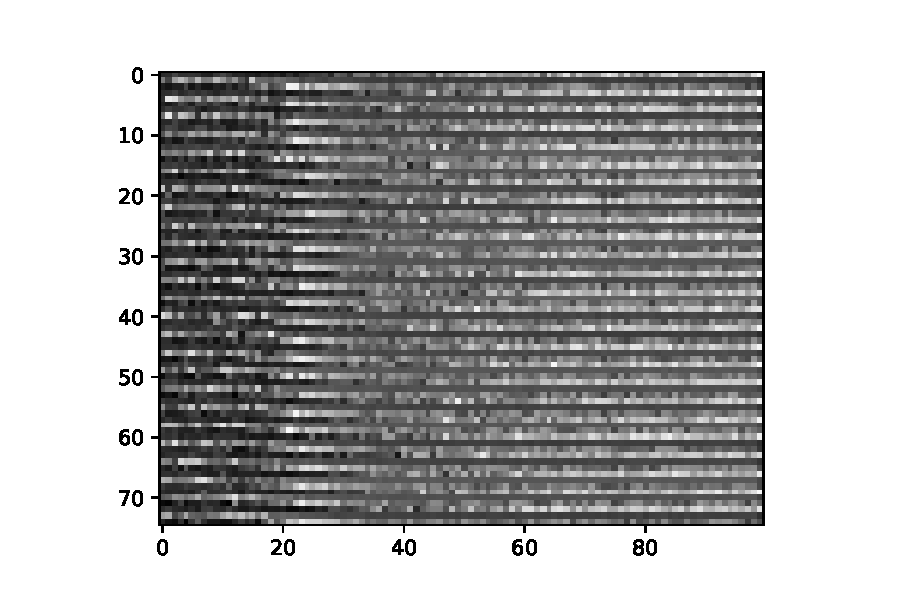
\includegraphics[width=0.7\textwidth]{weightswrong}
\caption{The weight matrix of the final fully connected layer after 1000 epochs. The phase transistion has become less defined compared the weight matrix after 300 epochs from figure \ref{fig:weightscnn}. \label{fig:weightswrong}}
\end{figure}

\begin{figure}[H]
\centering
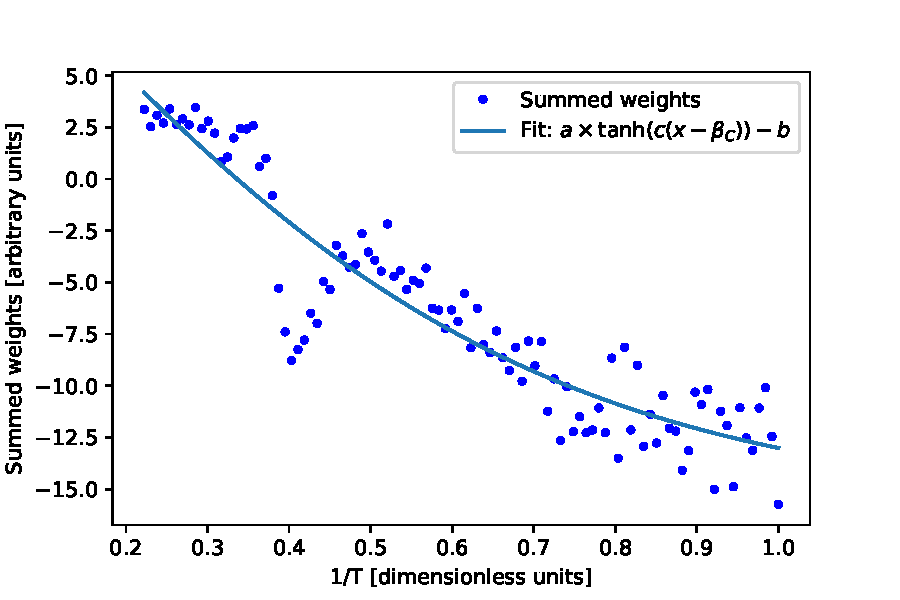
\includegraphics[width=0.7\textwidth]{fitwrong}
\caption{Sum of the weights for each of the classes with the fitted $\tanh$ function for the weight matrix after 1000 epochs. The phase tranistion has become less defined than for the weight matrix after 300 epochs in figure \ref{fig:fit}. The fit fails to properly fit the data. \label{fig:fitwrong}}
\end{figure}

The fitted $\tanh$ function does not properly fit this data and therefore the prediction is makes for the critical temperature does not represent the actual critical temperature. This fit parameter could however be used to observe how the network evolves after a number of epochs. In figure \ref{fig:epochs} we see the value of $\beta_C$ vs. the number of epochs. After about 500 epochs the network diverges away from the analytical value of $B_C$ denoted by the black line.


\begin{figure}[H]
\centering
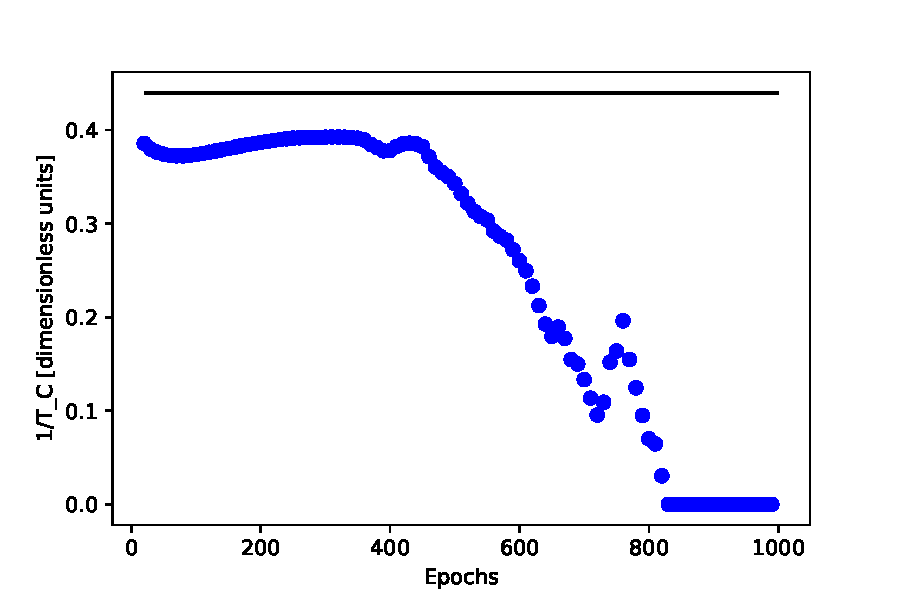
\includegraphics[width=0.7\textwidth]{epochs}
\caption{The best estimate for the inverse critical temperature vs. the number of epochs the network has run for. The black line denotes the analytical value of the critical temperature. After about 500 epochs the system suffers from overfitting and diverges away from the analytical value. \label{fig:epochs}}
\end{figure}

\section{Conclusion}


We used the metropolis algorithm to simulate the ferromagnetic zero field 2D square lattice Ising model and found that the behaviour of the magnetization per spin agrees with the expectation for a ferromagnetic system. It tends to $\pm 1$ for low temperatures and goes to 0 at higher temperatures with a clear phase transition at a finite temperature. For a system with a phase transition we expect the specific heat to have a peak at the critical temperature that becomes sharper as we tend towards the thermodynamic limit which is what we found. For a ferromagnetic system we expect the susceptibility to go to zero above and below the critical temperature with a peak at the critical temperature that becomes sharper as we approach the thermodynamic limit which is what we found. These results also agree with the results found in literature \cite{thijssen}.
\\
\\
Using a convolutional network we found a value for the critical temperature of $k_B T_C / J = 2.23(5)$ which agrees with the analytical result of $k_B T_C / J = \frac{2}{\ln(1 + \sqrt{2})} \simeq 2.2691 \dots $. The network used for the determination of the critical temperature classifies the temperature with an accuracy of 25\%. Running the network for more epochs produces a higher accuracy but reduces the definition of the phase transition in the weight matrix of the final layer. This might be due to over fitting, in order to evaluate whether this is the case a bigger dataset would need to be generated and the network run again. This might produce a value of $T_C$ with a smaller uncertainty.

\begin{thebibliography}{99}

\bibitem{thijssen} 
J.M. Thijssen (2013), \textit{Computational Physics}, Cambridge University Press, Cambridge, UK.

\bibitem{onsager}
L. Onsager (1944), \textit{"Crystal statistics. I. A two-dimensional model with an order-disorder transition"}, Physical Review, Series II, 65 (3–4): 117–149.

\bibitem{deep}
J. Patterson \& A. Gibson (2017), \textit{Deep Learning: A Practitioner's Approach}, O'Reilly Media, Sebastopol (CA.), USA.

\bibitem{IsingRBM}
G. Torial \& R.G. Meiko (2016), \textit{Learning thermodynamics with Boltzmann machines}, Phys. Rev. B 94, 165134.



\bibitem{phasemethod}
A. Tanaka \& A. Tomiya (2017), \textit{Detection of Phase Transition via Convolutional Neural Networks}, Journal of the Physical Society of Japan 86, 063001.


\end{thebibliography}

\end{document}